\documentclass[numbers=noenddot,12pt,a4paper]{scrartcl}
\usepackage[greek,ngerman]{babel}
\usepackage[T1]{fontenc}
\usepackage[utf8]{inputenc}
\usepackage{fullpage}
\usepackage{libertine}
\usepackage{ziffer}
\usepackage{graphicx}
\usepackage{units}
\usepackage[infoshow]{tabularx}
\usepackage{amsmath}
\usepackage{amssymb}
\usepackage{wrapfig}
\usepackage{esint}
\usepackage{float}
\usepackage{wrapfig}
\usepackage[font=small]{caption}
\usepackage{subcaption}
\usepackage{lscape}

\renewcommand{\thefigure}{Abb. \arabic{figure}}

\captionsetup[wrapfigure]{name=}
\captionsetup[figure]{name=}
\newcommand{\degree}{^\circ}
\newcommand{\diff}{\textnormal{d}}
\newcommand{\tenpo}[1]{\cdot 10^{#1}}
\newcommand{\greek}[1]{\greektext#1\latintext}
\newcommand{\ix}[1]{_\text{#1}}
\newcommand{\imag}{\mathbf{i}}

\title{Protokoll: Nanoparticle Tracking}
\author{Tom Kranz, Philipp Hacker}
\date{\today}

\begin{document}
%\setcounter{page}{2}
%\setcounter{section}{1}
\maketitle
\begin{center}
Betreuer: M. Paßvogel\\
Versuchsdatum: 21.10.2014\\
\begin{table}[h]
\centering
Note:
\begin{tabularx}{1.5cm}{|X|}
\hline \\ \\
\hline
\end{tabularx}
\end{table}
\end{center}
\vspace*{\fill}
\tableofcontents
\vfill
\newpage
\section{Einleitung}
Der Versuch "`Nanoparticle Tracking"' befasst sich mit der Detektion von Nanopartikeln in Lösungen und der Messung ihrer Eigenschaften, unter anderem ihrer Größe und ihres Diffusionskoeffizienten. Dazu wird ein System der Firma \textsc{NanoSight Ltd.} benutzt, das im Abschnitt \ref{kap:durchf} näher beschrieben wird. Nanopartikel sind Verbünde einer relativ geringen Anzahl von Atomen oder Molekülen, die durch ihre Größe, meist im Nanometer-Bereich, charakterisiert sind. 
\section{Physikalische Grundlagen}
\subsection{Diffusion}
Die ungerichtete thermische Bewegung von Atomen, Ionen und Molekülen in Medien, die Translationsbewegungen zulassen, bewirkt eine Durchmischung ursprünglich inhomogener Stoffgemische bis zum Zustand völliger Homogenität. Diese Bewegung wird "`Brownsche Bewegung"' genannt und der Vorgang der Durchmischung "`Diffusion"'. Obgleich die Brownsche Bewegung stets ungerichtet ist, lässt sich eine Abhängigkeit der Stärke der Diffusion vom Konzentrationsgefälle des betrachteten Stoffs im Medium feststellen. Diese manifestiert sich in einem linearen Zusammenhang zwischen durch Diffusion bedingte Teilchenstromdichte $\vec{j}$ und dem Gradienten des Konzentrationsprofils $\vec{\nabla} c(\vec{r},t)$. Da der Gradient immer in Richtung Maximum zeigt und Teilchen durch Diffusion von hochkonzentrierten in niederkonzentrierte Bereiche gespült werden, ergibt sich folgende Beziehung, das erste Ficksche Gesetz:
\begin{align}\label{eq:grad}
\vec{j}=-D\cdot\vec{\nabla}c
\end{align}
mit dem Diffusionskoeffizienten $D$. Die Existenz einer Teilchenstromdichte bedingt direkt eine lokale Änderung der Konzentration; gibt es einen Ort, aus dem $\vec{j}$ entspringt, bedeutet dies, dass von dort Teilchen wegfließen und die Konzentration dementsprechend abnimmt. Dies wird ausgedrückt über die Divergenz von $\vec{j}\left(\vec{r}\right)$ im zweiten Fickschen Gesetz:
\begin{align}
\frac{\partial c}{\partial t}&=-\vec{\nabla}\circ\vec{j}\\
&=-\vec{\nabla}\circ(-D\cdot\vec{\nabla} c)=D\cdot\vec{\nabla}^2c=D\cdot\left[\frac{\partial^2}{\partial x^2}+\frac{\partial^2}{\partial y^2}+\frac{\partial^2}{\partial z^2}\right]c\label{eq:bew}
\end{align}
Die mit Gleichung (\ref{eq:bew}) beschriebene partielle Differentialgleichung beinhaltet die Dynamik des Konzentrationsprofils $c(\vec{r},t)$.
\subsection{Stokessches Gesetz}
Die Bewegung von Nanopartikeln durch Flüssigkeiten kann mit der einer Kugel mit Radius $r\ix{P}$ und entsprechendem Volumen $V\ix{P}$ verglichen werden: Es wirken die Gravitationskraft $\vec{F}\ix{G}=m\ix{P}\cdot\vec{g}$, die Auftriebskraft $\vec{F}\ix{B}=-\rho\ix{M}\cdot V\ix{P}\cdot\vec{g}$ und die Reibungskraft (nach Stokes)\linebreak$\vec{F}\ix{F}=-6\cdot\pi\cdot r\ix{P}\cdot\eta\cdot\vec{u}$ mit $m\ix{P}$ der Partikelmasse, $\vec{g}$ der Erdbeschleunigung, $\rho\ix{M}$ der Massendichte des Mediums, $\eta$ der Viskosität des Mediums, $\vec{u}=\frac{\diff \vec{r}}{\diff t}$.
\subsection{Stokes-Einstein-Gleichung}
Eine Betrachtung der Teilchenstrombilanz liefert:
\begin{align}
c(\vec{r},t)\cdot\vec{u}+\vec{j}(\vec{r},t)=0
\end{align}
Einsetzen von $\vec{u}$ aus $\vec{F}\ix{F}$ und Gleichung (\ref{eq:grad}) führt zu
\begin{align}
\frac{\vec{F}\ix{F}\cdot c(\vec{r},t)}{6\cdot\pi\cdot\eta\cdot r\ix{K}}=D\cdot\vec{\nabla}c(\vec{r},t)\label{eq:stokes}
\end{align}
Durch Einbeziehung von Osmose, der Diffusion durch semipermeable Membranen, die durch einen osmotischen Druck $\Delta p$ gekennzeichnet ist, der auf ein von einer semipermeablen Membran umschlossenen Volumen einer Lösung wirkt, wenn es in reines Lösungsmittel getaucht wird. Der Druckunterschied ergibt sich zu $\Delta p=\rho\ix{M}\cdot g\cdot h$ mit $h$ dem Höhenunterschied des Füllstandes der Lösung durch den wirkenden Druck, wenn sich ein Kräftegleichgewicht zwischen osmotischer Kraft und den übrigen Kräften eingestellt hat. Das van't Hoffsche Gesetz stellt eine der idealen Gasgleichung ähnliche Aussage für Lösungen auf:
\begin{align}
p\cdot V=\nu\cdot R\cdot T
\end{align}
mit $\nu$ der Stoffmenge des gelösten Stoffs, $R$ der allgemeinen Gaskonstante und $T$ der Temperatur der Lösung. Wenn man nun $c=\frac{\nu\cdot N_A}{V}$ ($N_A$ ist die Avogadro-Zahl in $\unit{mol^{-1}}$) beachtet, ergibt sich für die osmotische Kraft:
\begin{align}
\vec{F}\ix{O}\cdot c(\vec{r},t)=\vec{\nabla} p=\frac{R\cdot T}{N_A}\cdot\vec{\nabla} c(\vec{r},t)\label{eq:osm}
\end{align}
Vergleich der Gleichungen (\ref{eq:stokes}) und (\ref{eq:osm}) zeigt, dass im Kräftegleichgewicht gilt:
\begin{align}
D=\frac{k_B\cdot T}{6\cdot\pi\cdot\eta\cdot r\ix{K}}
\end{align}
Mit der Boltzmann-Konstante $k_B=\frac{R}{N_A}$. Durch weitere Überlegung bezüglich der Wahrscheinlichkeit, ein Teilchen in einem bestimmten $x$-Intervall $\left[x;x+\diff x\right]$ zu finden, ergibt sich das mittlere Quadrat des von einem Teilchen zurückgelegten Weges zu:
\begin{align}
\left\langle x^2 \right\rangle(t)=2\cdot D\cdot t
\end{align}
Dieser Zusammenhang lässt eine schnelle Bestimmung von $D$ zu, wenn man die Trajektorien gelöster Partikel über einen gewissen Zeitraum beobachtet.
\section{Durchführung}\label{kap:durchf}

\section{Auswertung}
Die von \textbf{NTA} ausgebenen Dateien enthielten Daten zu einzelnen verfolgten Partikeln. Diese mussten von nicht relevanten Datensätzen (vom Programm als solche gekennzeichnet) und Mehrfachnennungen der übrigen Partikel befreit werden und konnten dann zur Erstellung von Histogrammen und zur grundlegenden statistischen Analyse benutzt werden. Das Ergebnis kann im Anhang betrachtet werden, wobei der Mittelwert der jeweils ausgewerteten Größe als schwarze Linie und die einfache Standardabweichung als graue Umgebung gekennzeichnet sind. Für die durchschnittlichen Partikeldurchmesser des Automaten- und des Maschinenkaffees wurden die jeweils berechneten Mittelwerte und ihre Standardabweichungen untereinander gemittelt, wobei Werte, die aus längeren Messungen stammen, eine höhere Gewichtung zukam. Für die Diffusionskoeffizienten wurden die Mittelwerte bei gleicher Konzentration benutzt, da die Verdünnung Einfluss auf diese Größe hat.
\begin{align*}
%	\overline{d}\ix{Automat}&=\unit[\left(134\pm 83\right)]{nm} \\
%	\overline{D}\ix{A, 1:9}&=\unit[\left(2,5\pm 1,1 \right)]{\frac{\mu m^2}{s}} \\
%	\overline{d}\ix{Maschine}&=\unit[\left(137\pm 72\right)]{nm} \\
%	\overline{D}\ix{M, 1:4}&=\unit[\left(8,0\pm 5,0\right)]{\frac{\mu m^2}{s}} \\
%	\overline{D}\ix{M, 1:9}&=\unit[\left(4,3\pm 2,3\right)]{\frac{\mu m^2}{s}} \\
%	\overline{D}\ix{M, 1:19}&=\unit[\left(5,1\pm 3,0\right)]{\frac{\mu m^2}{s}} \\
\begin{array}{c|c|c|c|c|c}
\unit[\overline{d}\ix{Automat}]{/nm}& \unit[\overline{D}\ix{A, 1:9}]{/\frac{\mu m^2}{s}} & \unit[\overline{d}\ix{Maschine}]{/nm} & \unit[\overline{D}\ix{M, 1:4}]{/\frac{\mu m^2}{s}} & \unit[\overline{D}\ix{M, 1:9}]{/\frac{\mu m^2}{s}} & \unit[\overline{D}\ix{M, 1:19}]{/\frac{\mu m^2}{s}} \\
\hline 
\left(134\pm 83\right)	& \left(2,5\pm 1,1 \right) & \left(137\pm 72\right) & \left(8,0\pm 5,0\right) & \left(4,3\pm 2,3\right) & \left(5,1\pm 3,0\right)
\end{array} 
\end{align*}
Beim Betrachten der Histogramme fällt die große Standardabweichung im Verhältnis zum Mittelwert auf. Auch sticht ins Auge, dass ein klassischer Mittelwert der Messverteilung nicht gerecht wird, da dieser sich teilweise bereits weit auf der abfallenden Flanke der Verteilung befindet, während sich die Messungen um einen anderen Wert häufen. Eine genauere Analyse der Messwertverteilungen wäre daher angebracht, um eventuell genauere Werte zu gewinnen -- momentan wird der Ungenauigkeit durch einen großen Messfehler (Standardabweichung) Rechnung getragen.\\
Das Programm selbst bietet eine Zusammenfassung der gemessenen Daten an, jedoch gibt diese unter Umständen verschiedene Größen aus und die Werte für die ausgegebenen Größen liegen weit außerhalb der Möglichkeiten des Messwertspektrums.\\
Zu Fehlerquellen in der Messung liegen uns keine relevanten Informationen vor, da die gesamte Messapparatur ein proprietäres Design darstellt und keinen Einblick in die Messungen zulässt; die Auswertung erfolgt allein über die ausgegebenen Daten der zugehörigen Software. Es lassen sich aber externe Faktoren erahnen, welche mehr oder weniger starken Einfluss auf die Messungen haben könnten: Vibrationen des Experimentiertisches, Teperaturschwankungen (die Messung findet unter der Vorraussetzung einer konstanten Temperatur statt), Verunreinigungen der untersuchten Suspension und der optischen Bauteile des Aufbaus.
\section{Anhang}
\subsection{Messwerte}
\begin{landscape}
	\begin{figure}[H]
		\hspace{-3cm}
		\begin{subfigure}[b]{0.85\textwidth}
			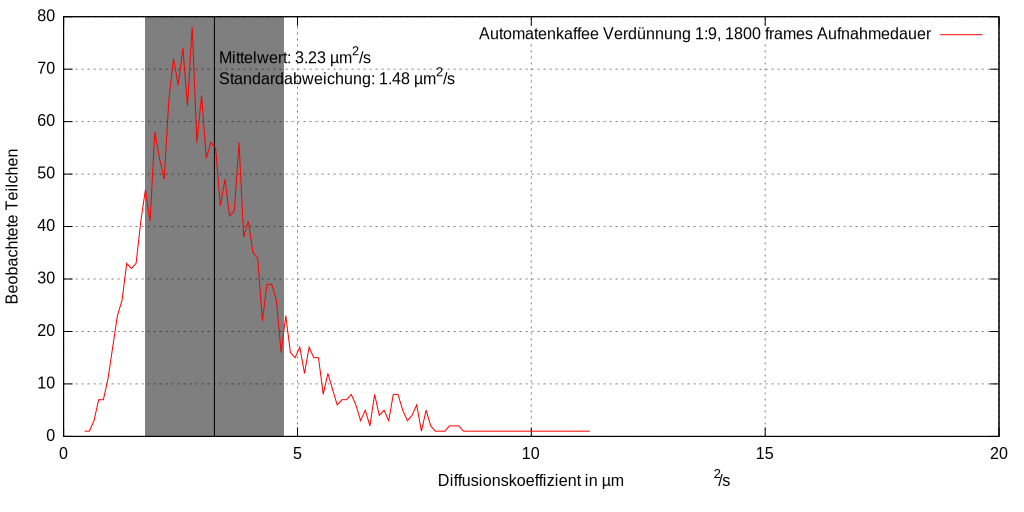
\includegraphics[width=\textwidth]{{messwerte/cleaned/kaffeeautomat-001-alltracks.diffco}.pdf}
		\end{subfigure}
		\begin{subfigure}[b]{0.85\textwidth}
			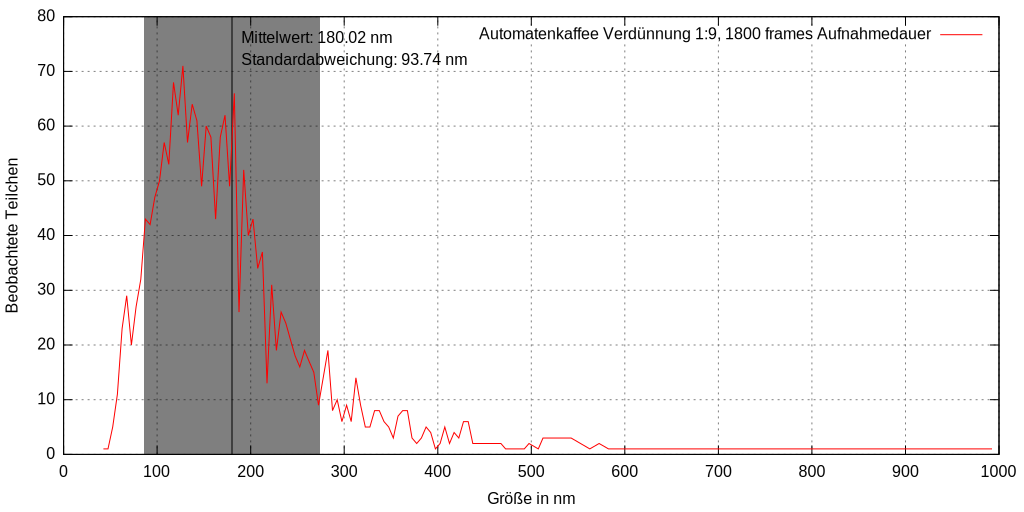
\includegraphics[width=\textwidth]{{messwerte/cleaned/kaffeeautomat-001-alltracks}.pdf}
		\end{subfigure}
	\end{figure}
	\vspace{1cm}
	\begin{figure}[H]
		\hspace{-3cm}
		\begin{subfigure}[b]{0.85\textwidth}
			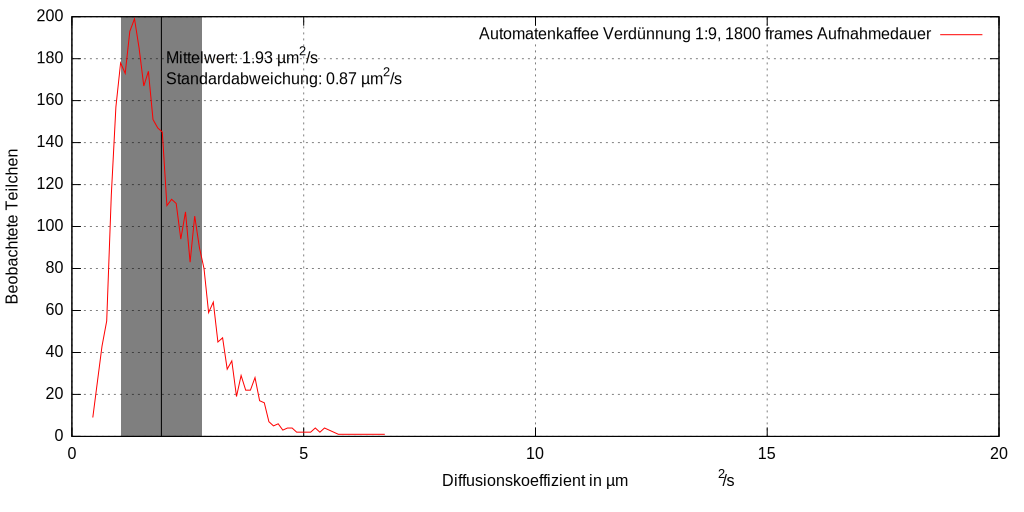
\includegraphics[width=\textwidth]{{messwerte/cleaned/kaffeeautomat2-001-alltracks.diffco}.pdf}
		\end{subfigure}
		\begin{subfigure}[b]{0.85\textwidth}
			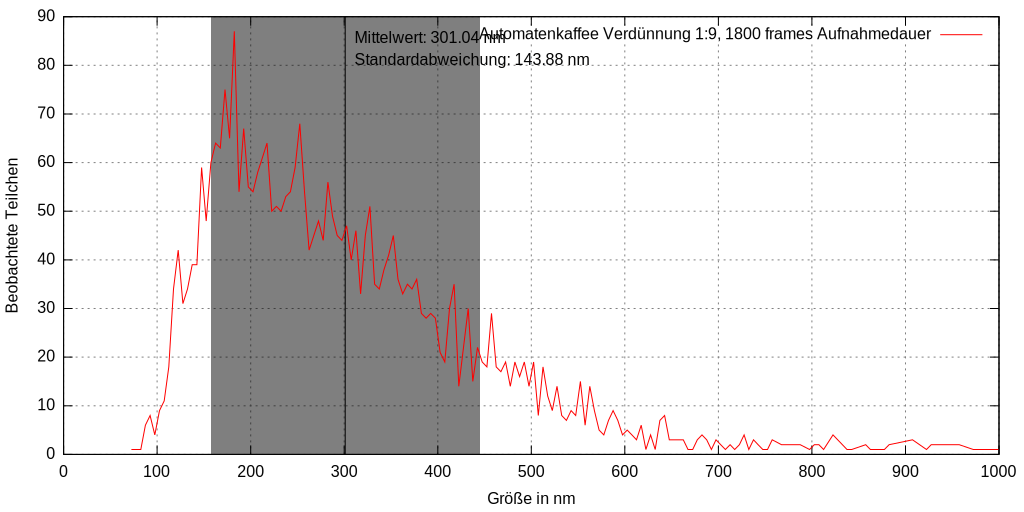
\includegraphics[width=\textwidth]{{messwerte/cleaned/kaffeeautomat2-001-alltracks}.pdf}
		\end{subfigure}
	\end{figure}
	\begin{figure}[H]
		\hspace{-3cm}
		\begin{subfigure}[b]{0.85\textwidth}
			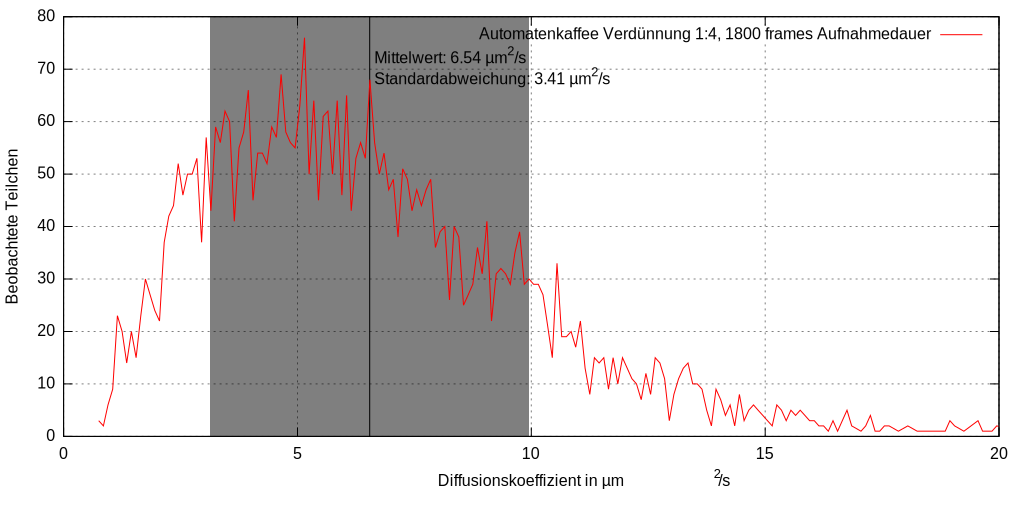
\includegraphics[width=\textwidth]{{messwerte/cleaned/kaffeeautomat3-001-alltracks.diffco}.pdf}
		\end{subfigure}
		\begin{subfigure}[b]{0.85\textwidth}
			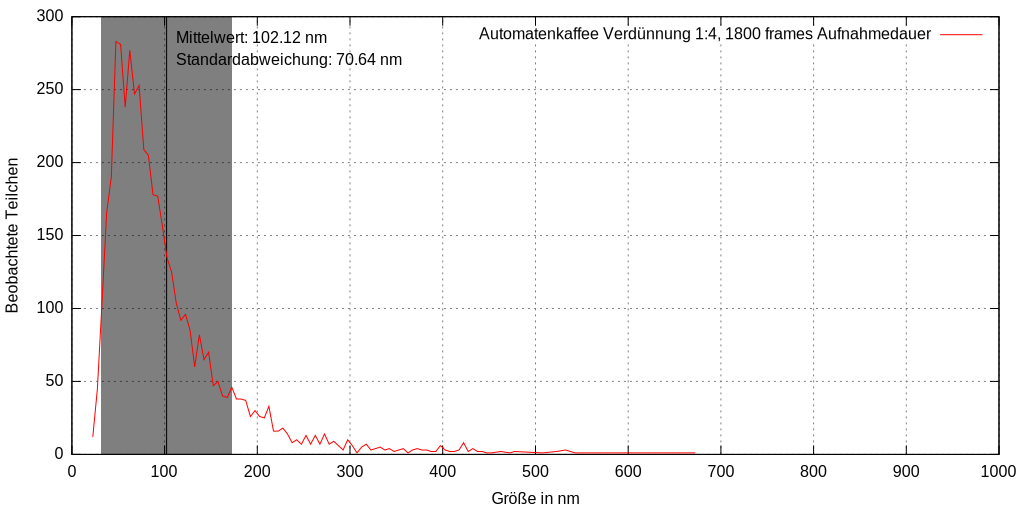
\includegraphics[width=\textwidth]{{messwerte/cleaned/kaffeeautomat3-001-alltracks}.pdf}
		\end{subfigure}
	\end{figure}
	\vspace{1cm}
	\begin{figure}[H]
		\hspace{-3cm}
		\begin{subfigure}[b]{0.85\textwidth}
			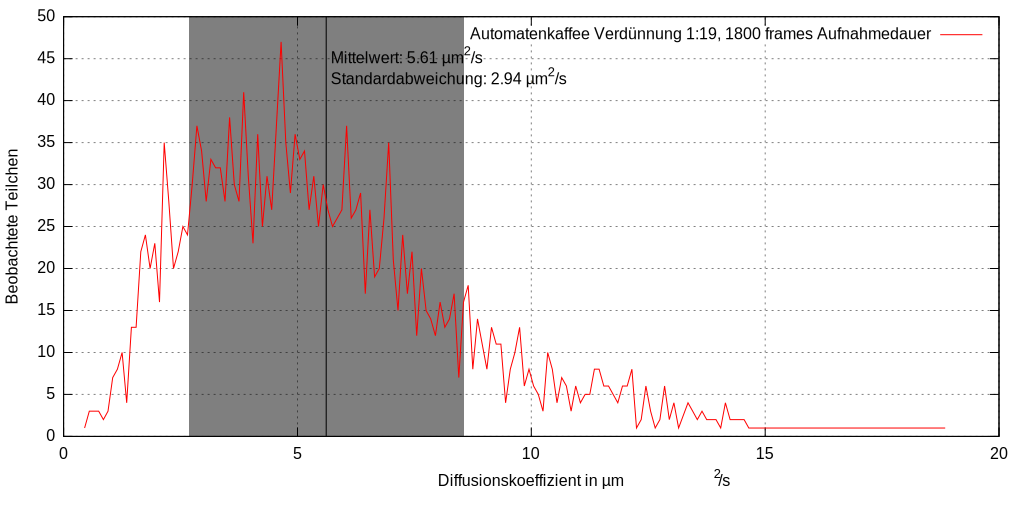
\includegraphics[width=\textwidth]{{messwerte/cleaned/kaffeeautomat4-001-alltracks.diffco}.pdf}
		\end{subfigure}
		\begin{subfigure}[b]{0.85\textwidth}
			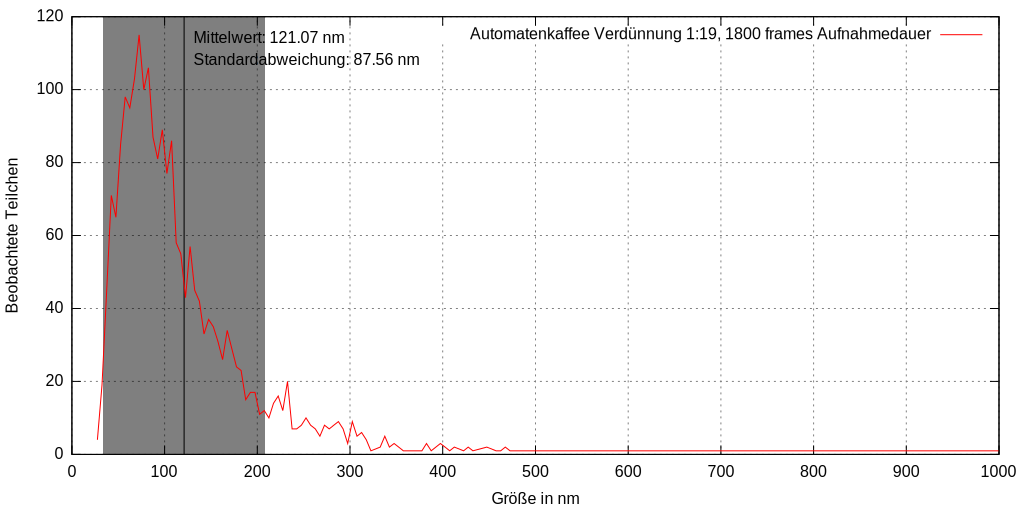
\includegraphics[width=\textwidth]{{messwerte/cleaned/kaffeeautomat4-001-alltracks}.pdf}
		\end{subfigure}
	\end{figure}
	\begin{figure}[H]
		\hspace{-3cm}
		\begin{subfigure}[b]{0.85\textwidth}
			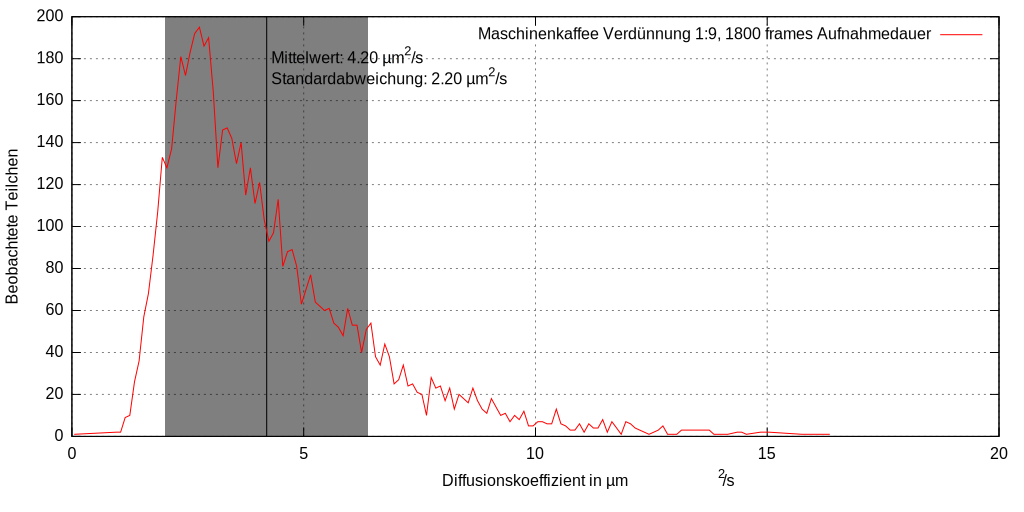
\includegraphics[width=\textwidth]{{messwerte/cleaned/kaffeemaschine-001-alltracks.diffco}.pdf}
		\end{subfigure}
		\begin{subfigure}[b]{0.85\textwidth}
			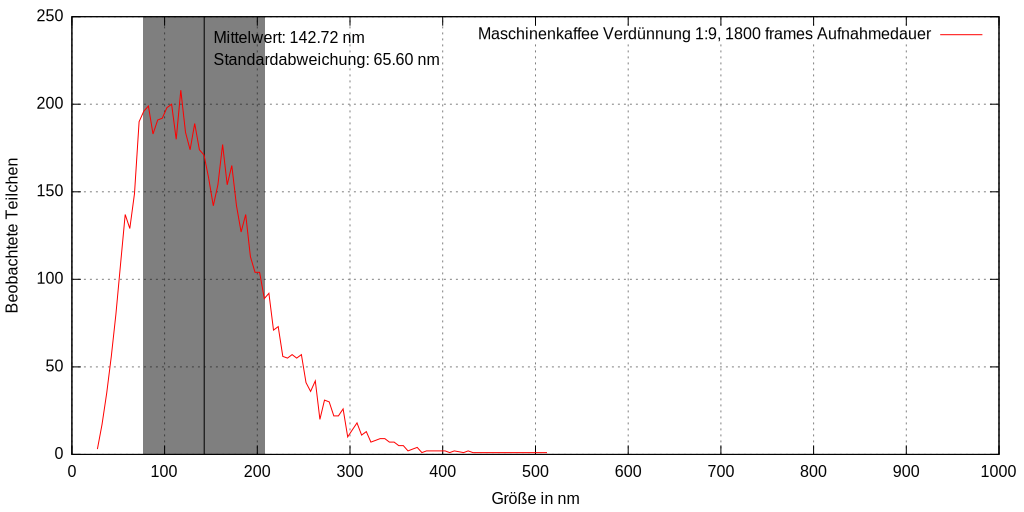
\includegraphics[width=\textwidth]{{messwerte/cleaned/kaffeemaschine-001-alltracks}.pdf}
		\end{subfigure}
	\end{figure}
	\vspace{1cm}
	\begin{figure}[H]
		\hspace{-3cm}
		\begin{subfigure}[b]{0.85\textwidth}
			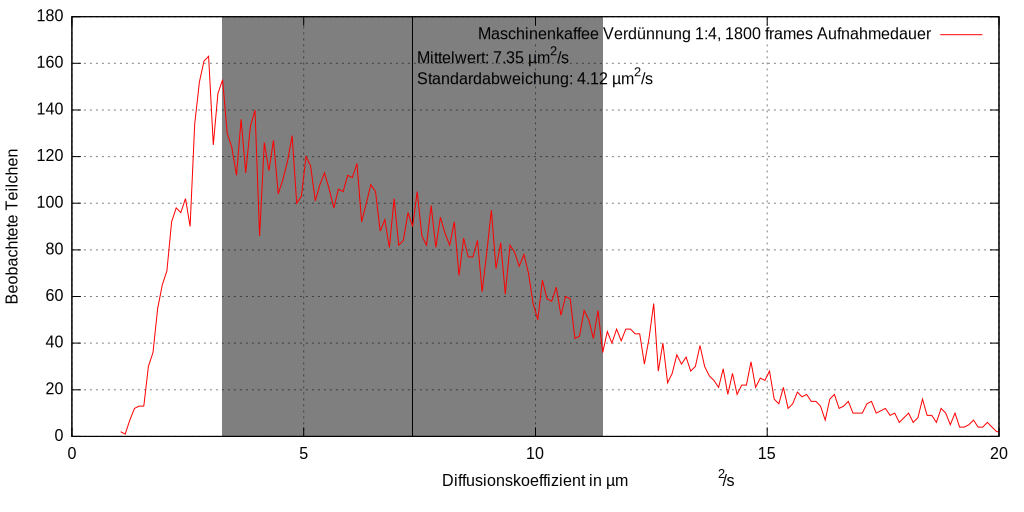
\includegraphics[width=\textwidth]{{messwerte/cleaned/kaffeemaschine2-001-alltracks.diffco}.pdf}
		\end{subfigure}
		\begin{subfigure}[b]{0.85\textwidth}
			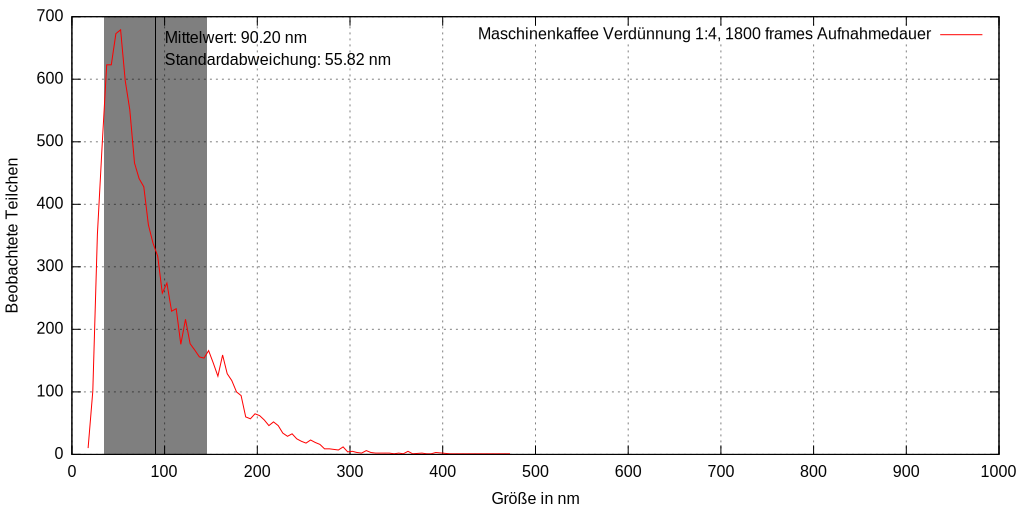
\includegraphics[width=\textwidth]{{messwerte/cleaned/kaffeemaschine2-001-alltracks}.pdf}
		\end{subfigure}
	\end{figure}
	\begin{figure}[H]
		\hspace{-3cm}
		\begin{subfigure}[b]{0.85\textwidth}
			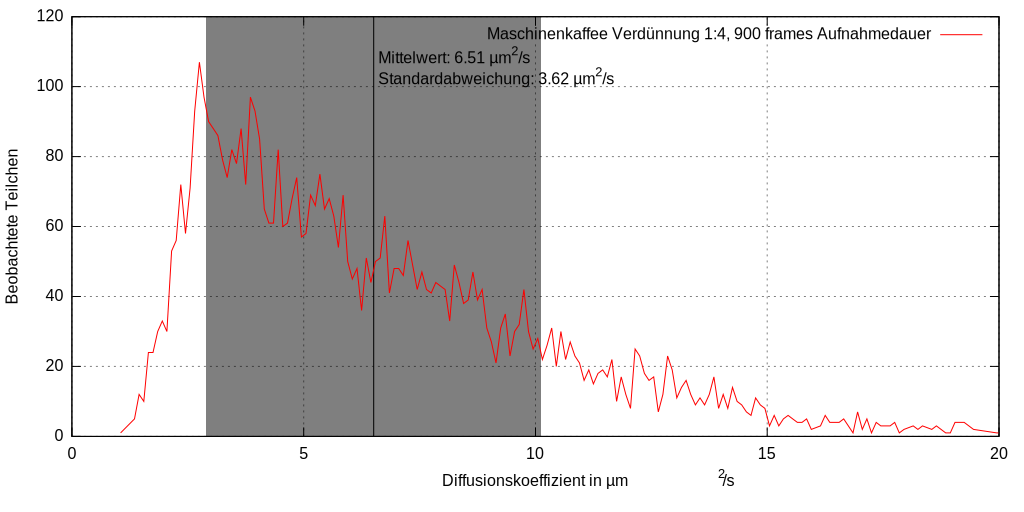
\includegraphics[width=\textwidth]{{messwerte/cleaned/kaffeemaschine2kurz-004-alltracks.diffco}.pdf}
		\end{subfigure}
		\begin{subfigure}[b]{0.85\textwidth}
			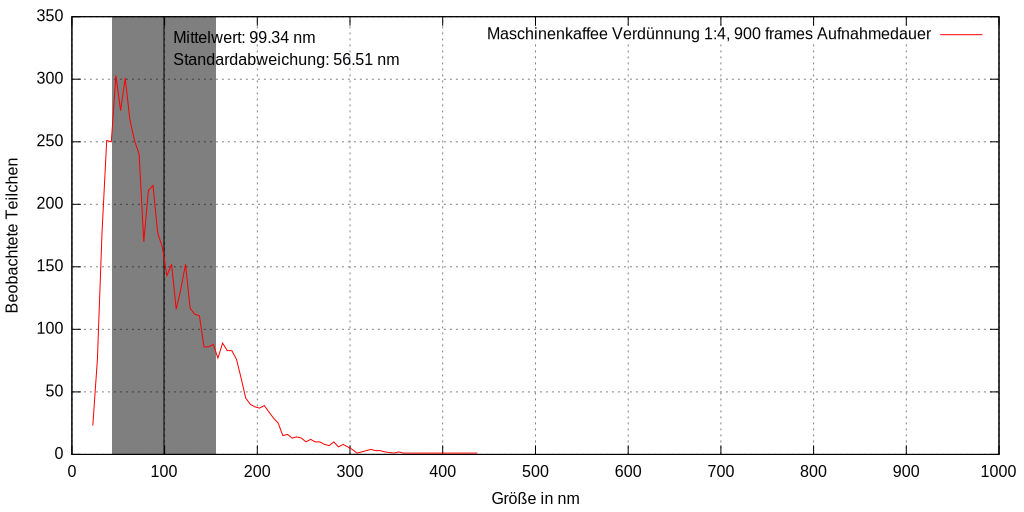
\includegraphics[width=\textwidth]{{messwerte/cleaned/kaffeemaschine2kurz-004-alltracks}.pdf}
		\end{subfigure}
	\end{figure}
	\vspace{1cm}
	\begin{figure}[H]
		\hspace{-3cm}
		\begin{subfigure}[b]{0.85\textwidth}
			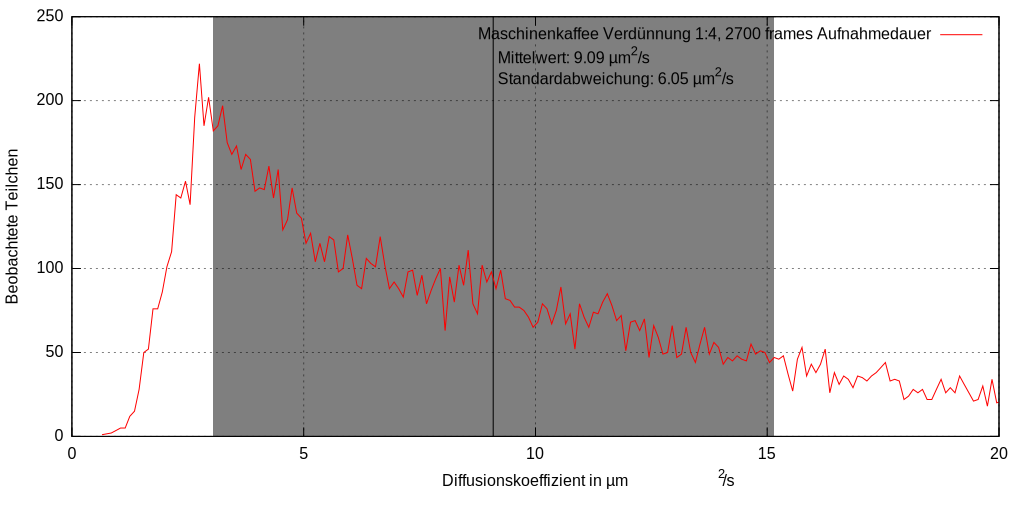
\includegraphics[width=\textwidth]{{messwerte/cleaned/kaffeemaschine2lang-001-alltracks.diffco}.pdf}
		\end{subfigure}
		\begin{subfigure}[b]{0.85\textwidth}
			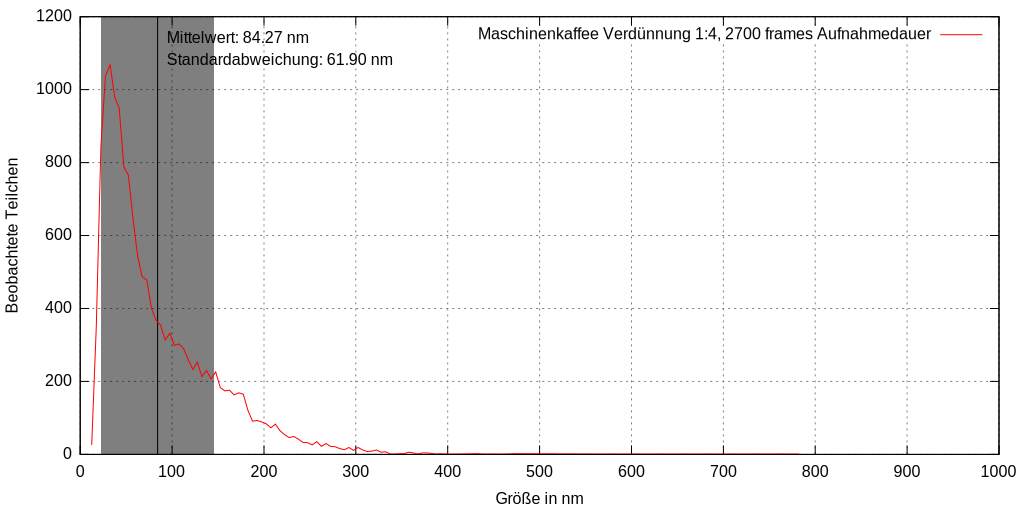
\includegraphics[width=\textwidth]{{messwerte/cleaned/kaffeemaschine2lang-001-alltracks}.pdf}
		\end{subfigure}
	\end{figure}
	\begin{figure}[H]
		\hspace{-3cm}
		\begin{subfigure}[b]{0.85\textwidth}
			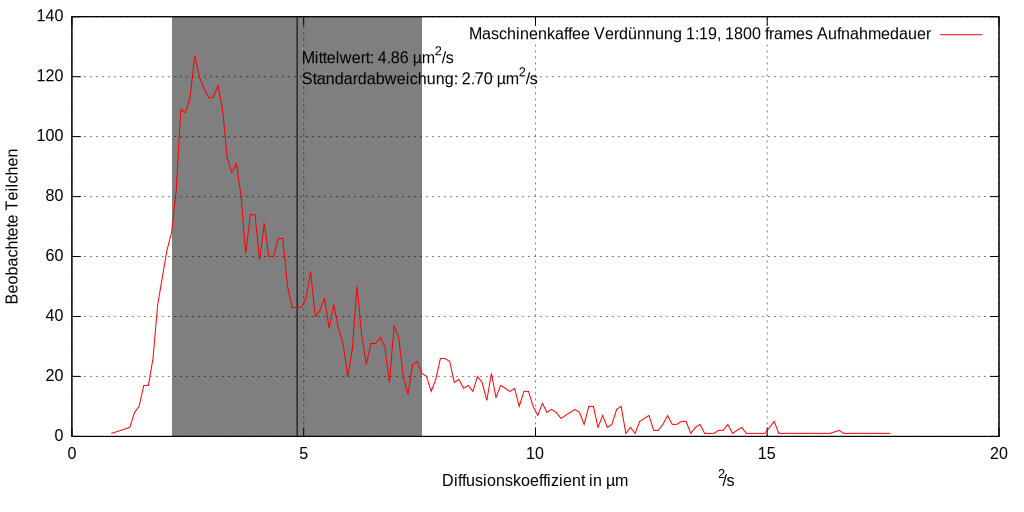
\includegraphics[width=\textwidth]{{messwerte/cleaned/kaffeemaschine3-001-alltracks.diffco}.pdf}
		\end{subfigure}
		\begin{subfigure}[b]{0.85\textwidth}
			\includegraphics[width=\textwidth]{{messwerte/cleaned/kaffeemaschine3-001-alltracks}.pdf}
		\end{subfigure}
	\end{figure}
	\vspace{1cm}
	\begin{figure}[H]
		\hspace{-3cm}
		\begin{subfigure}[b]{0.85\textwidth}
			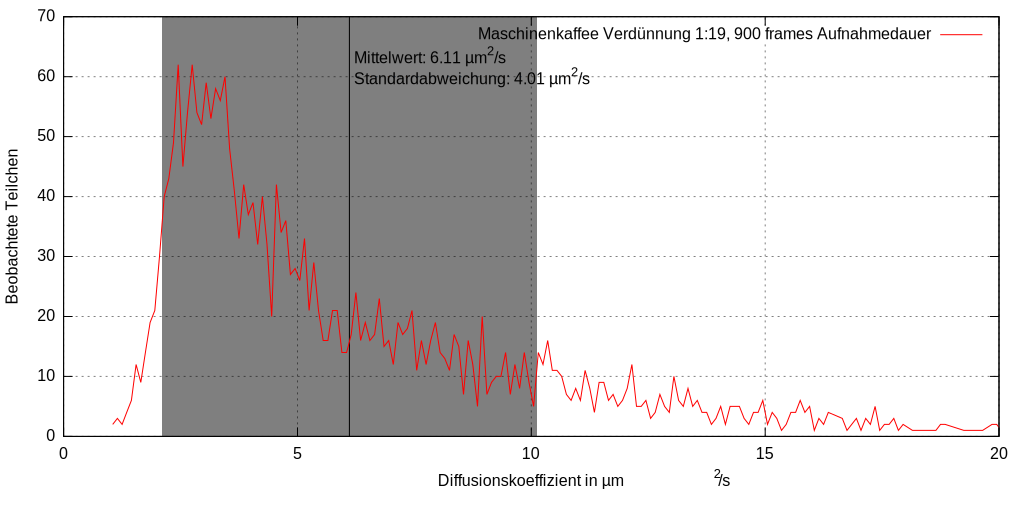
\includegraphics[width=\textwidth]{{messwerte/cleaned/kaffeemaschine3kurz-001-alltracks.diffco}.pdf}
		\end{subfigure}
		\begin{subfigure}[b]{0.85\textwidth}
			\includegraphics[width=\textwidth]{{messwerte/cleaned/kaffeemaschine3kurz-001-alltracks}.pdf}
		\end{subfigure}
	\end{figure}
	\begin{figure}[H]
		\hspace{-3cm}
		\begin{subfigure}[b]{0.85\textwidth}
			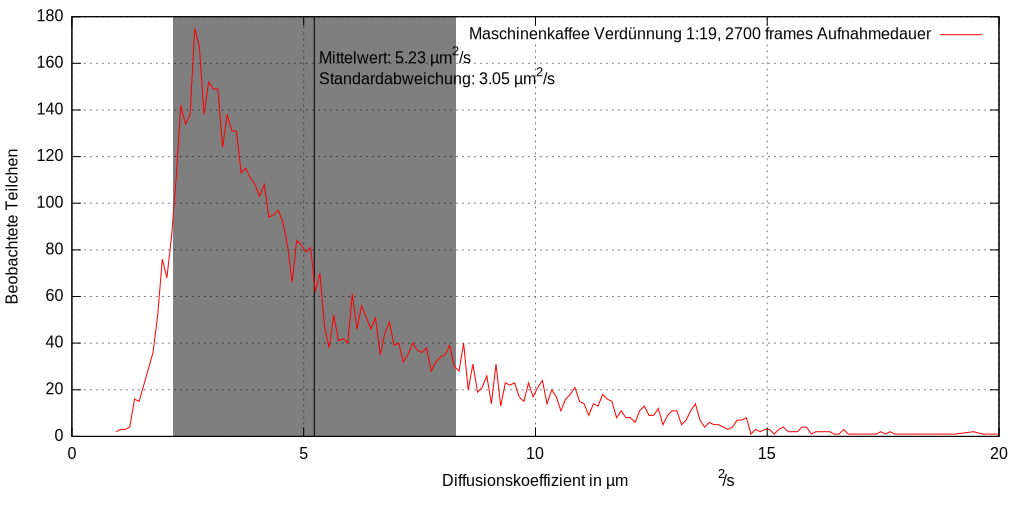
\includegraphics[width=\textwidth]{{messwerte/cleaned/kaffeemaschine3lang-001-alltracks.diffco}.pdf}
		\end{subfigure}
		\begin{subfigure}[b]{0.85\textwidth}
			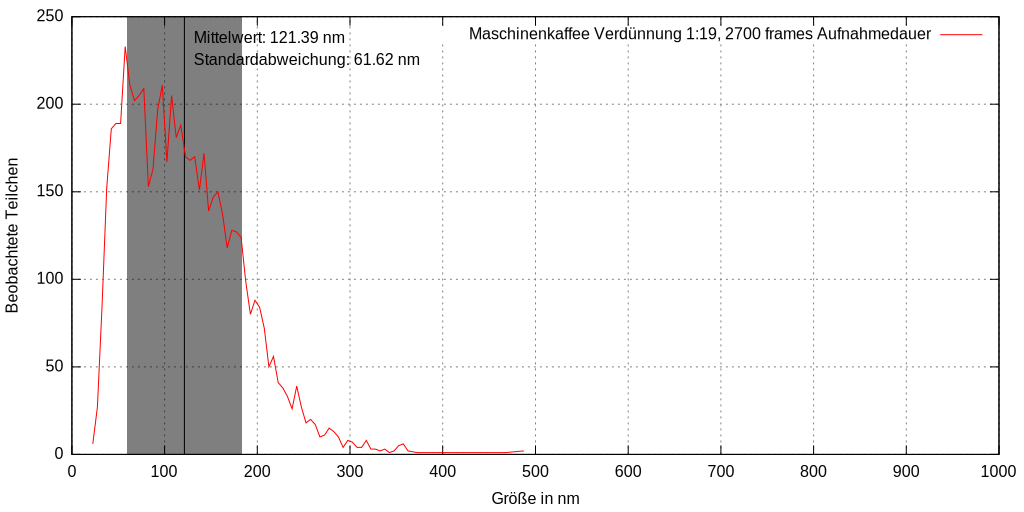
\includegraphics[width=\textwidth]{{messwerte/cleaned/kaffeemaschine3lang-001-alltracks}.pdf}
		\end{subfigure}
	\end{figure}
	\vspace{1cm}
	\begin{figure}[H]
		\hspace{-3cm}
		\begin{subfigure}[b]{0.85\textwidth}
			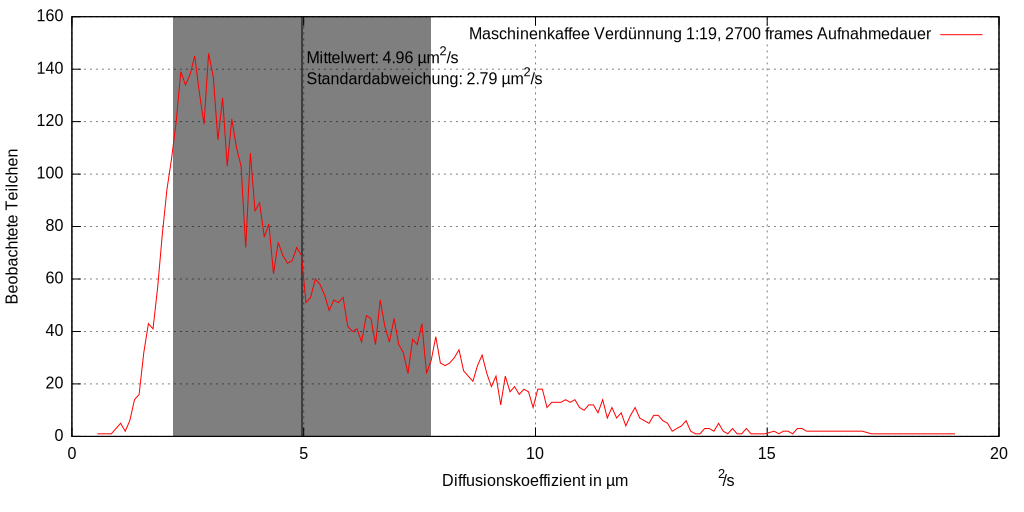
\includegraphics[width=\textwidth]{{messwerte/cleaned/kaffeemaschine3langkorrekt-001-alltracks.diffco}.pdf}
		\end{subfigure}
		\begin{subfigure}[b]{0.85\textwidth}
			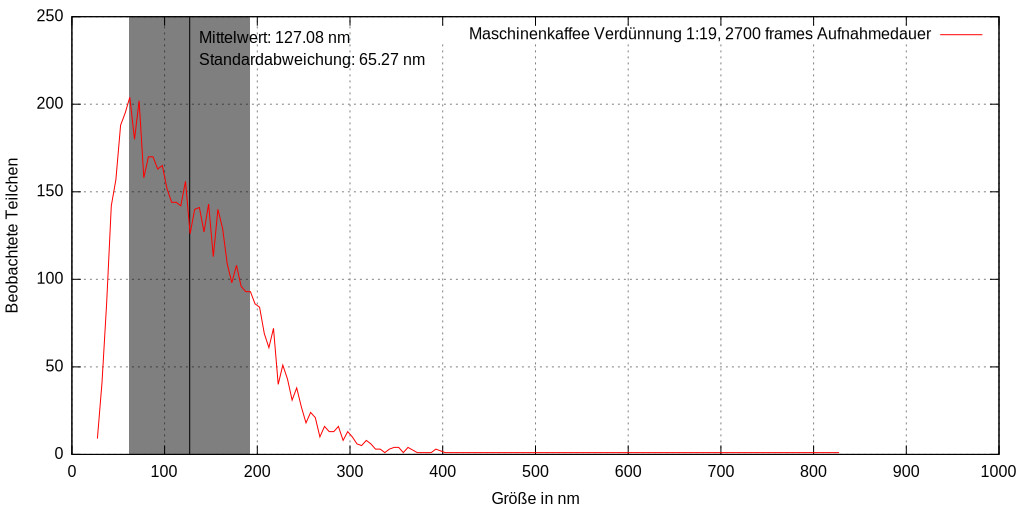
\includegraphics[width=\textwidth]{{messwerte/cleaned/kaffeemaschine3langkorrekt-001-alltracks}.pdf}
		\end{subfigure}
	\end{figure}
	\begin{figure}[H]
		\hspace{-3cm}
		\begin{subfigure}[b]{0.85\textwidth}
			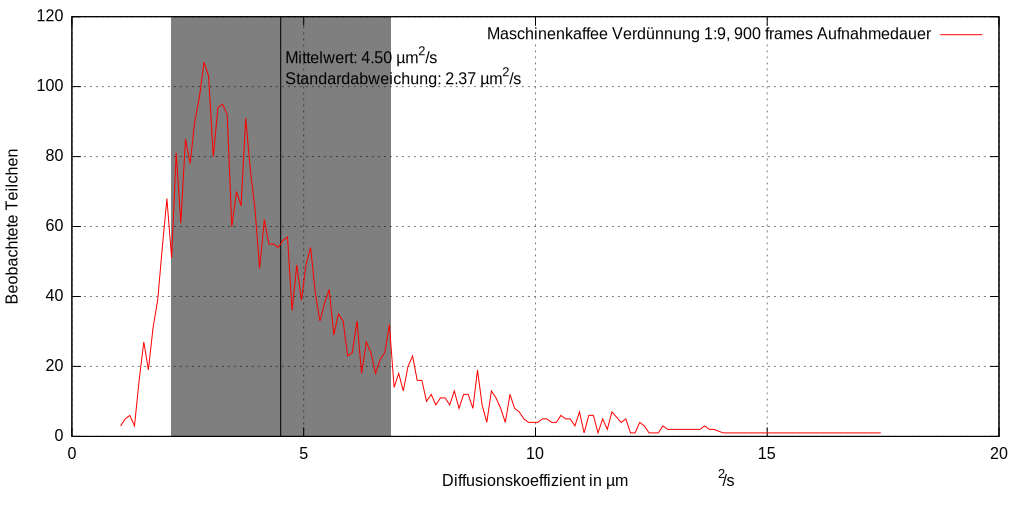
\includegraphics[width=\textwidth]{{messwerte/cleaned/kaffeemaschinekurz-001-alltracks.diffco}.pdf}
		\end{subfigure}
		\begin{subfigure}[b]{0.85\textwidth}
			\includegraphics[width=\textwidth]{{messwerte/cleaned/kaffeemaschinekurz-001-alltracks}.pdf}
		\end{subfigure}
	\end{figure}
	\vspace{1cm}
	\begin{figure}[H]
		\hspace{-3cm}
		\begin{subfigure}[b]{0.85\textwidth}
			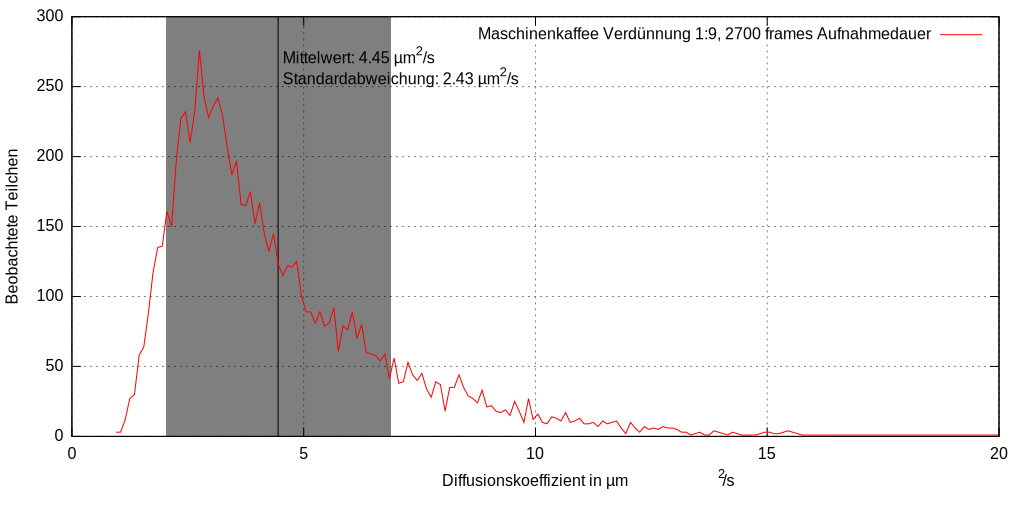
\includegraphics[width=\textwidth]{{messwerte/cleaned/kaffeemaschinelang-001-alltracks.diffco}.pdf}
		\end{subfigure}
		\begin{subfigure}[b]{0.85\textwidth}
			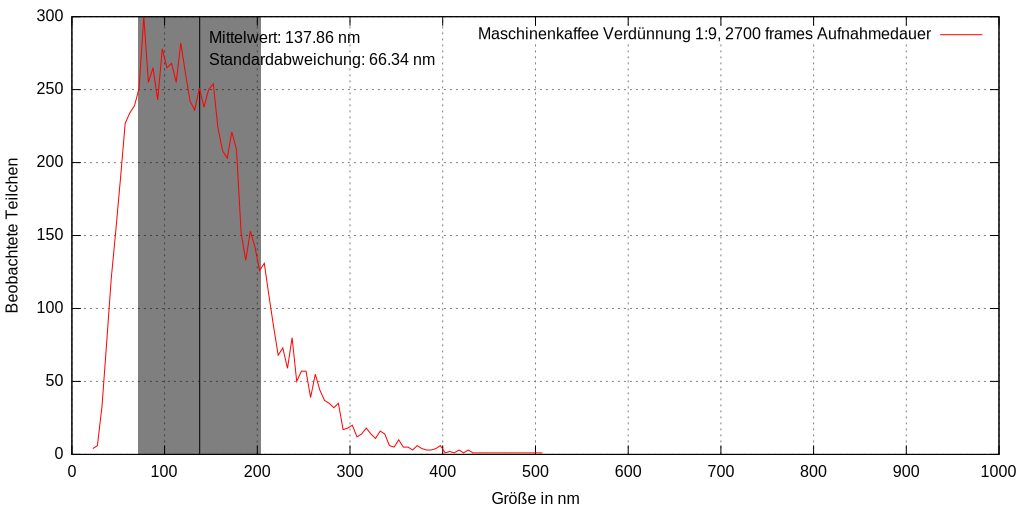
\includegraphics[width=\textwidth]{{messwerte/cleaned/kaffeemaschinelang-001-alltracks}.pdf}
		\end{subfigure}
	\end{figure}
\end{landscape}
\section{Anhang}
Die originalen Messwert-Aufzeichnungen liegen bei.
\end{document}